\begin{frame}{Τρωτά σημεία μεθόδων ευθυγράμμισης}

  \vspace{0.25cm}
  \noindent\makebox[0.65\linewidth][c]{%
  \begin{minipage}{0.5\linewidth}

    \begin{minipage}{0.3\linewidth}
      \begin{figure}
        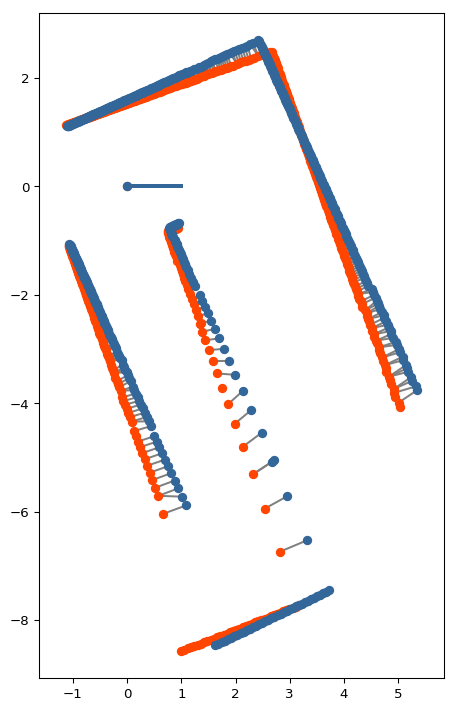
\includegraphics[scale=0.2]{./figures/slides/ch4/correspondence_is_the_culprit/pic0.png}
        \caption{\scriptsize Α}
      \end{figure}
    \end{minipage}
    \hfill
    \begin{minipage}{0.7\linewidth}
      \begin{figure}
        \animategraphics[scale=0.3,autoplay,loop]{1}{./figures/slides/ch4/correspondence_is_the_culprit/plicp/frame_}{0}{2}
        \caption{\scriptsize Β}
      \end{figure}
    \end{minipage} \\

  \begin{minipage}{\linewidth}
    \begin{figure}
      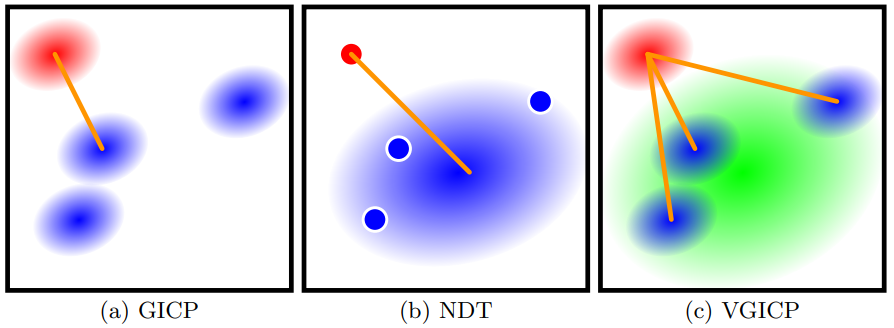
\includegraphics[scale=0.2]{./figures/slides/ch4/correspondence_is_the_culprit/gicp.png}
        \caption{\scriptsize Γ}
    \end{figure}
  \end{minipage}
  \end{minipage}
  }
  \noindent\makebox[0.3\linewidth][c]{%
    \begin{minipage}{0.3\linewidth}\scriptsize\vspace{-1cm}
    Α: ICP επί της αρχής (σημείο προς σημείο) \\

    Β: plicp: σημείο προς ευθύγραμμο τμήμα \\

    Γ: (a) Κατανομή προς κατανομή, (b) Σημείο προς κατανομή, (c) Κατανομή προς κατανομές \\\\

    \tiny
    Πηγές:\\
    Α:  Igor Bogoslavskyi, \url{https://nbviewer.org/github/niosus/notebooks/blob/master/icp.ipynb} \\

      B: A. Censi, ``An ICP variant using a point-to-line metric", \textit{IEEE International Conference on Robotics and Automation}, 2008, pp. 19-25 \\

      Γ: K. Koide, M. Yokozuka, S. Oishi and A. Banno, ``Voxelized GICP for Fast and Accurate 3D Point Cloud Registration", \textit{IEEE International Conference on Robotics and Automation}, 2021, pp. 11054-11059

  \end{minipage}
  }


\note{\footnotesize
Δεν είναι τυχαίο πως αυτά τα προβλήματα εμφανίζονται για τις παραμέτρους που
αφορούν στη διαδικασία εύρεσης αντιστοιχίσεων ανάμεσα στις ακτίνες των σαρώσεων
εισόδου. Αν ψάξει κανείς τη βιβλιογραφία θα ανακαλύψει μάλιστα ότι δεν υπάρχει
μέθοδος ευθυγράμμισης που να μην χρησιμοποιεί κάποιου είδους μηχανισμό
αντιστοίχισης, ο οποίος προσπαθεί να εκτιμήσει την αντιστοίχιση σημείων ή
κατανομών σημείων της μίας σάρωσης προς σημειο, ευθύγραμμο τμήμα, ή κατανομή
της άλλης.}

\end{frame}
